\subsection{\texorpdfstring{Applications: I. Duality of the spaces \(L^{p}\)}{Applications: I. Duality of the spaces L to the p}}

We shall treat here only the case of the real spaces \(\mathbf{L}^p\) .

Recall that two numbers \(p, q\) such that \(1 \leqslant p \leqslant +\infty\) , \(1 \leqslant q \leqslant +\infty\) , \(1/p + 1/q = 1\) are said to be conjugate exponents (Ch. IV, §6, No.~4). Every function \(g \in \mathcal{L}^q\) defines a continuous linear form \(\theta_g\) on \(L to the p\) , obtained by passing to the quotient starting with the linear form \(f \mapsto \int fg d\mu\) on \(\mathcal{L}^p\) , and one has \(N_q(g) = \| \theta_g \|\) (Ch. IV, §6, No.~4, Cor. of Prop. 3). Passing to the quotient, one thus deduces from the mapping \(g \mapsto \theta_g\) an isometric linear mapping \(\varphi\) of \(L^q\) into the dual \((L to the p)'\) of \(L to the p\) . We are going to show that, for \(1 \leqslant p < +\infty\) , \(\varphi\) maps \(L^q\) onto \((L to the p)'\) , so that we may henceforth identify the Banach space \(L^q\) with the Banach space \((L to the p)'\) by means of the isomorphism \(\varphi\) . Stated in other terms:

THEOREM 4. --- Let p and q be two conjugate exponents such that \(1 \leqslant p < +\infty\) . Every continuous linear form on \(\mathcal{L}^{p}(\mathrm{T}, \mu)\) is of the type \(f \mapsto \int fg d\mu\) , where g is a function in \(\mathcal{L}^{q}(\mathrm{T}, \mu)\) whose class in \(L^{q}\) is well-defined.

Let \(\theta\) be a continuous linear form on \(\mathcal{L}^p\) ; thus, there exists a number \(a \geqslant 0\) such that \(|\theta(f)| \leqslant a \cdot \mathrm{N}_p(f)\) for every function \(f \in \mathcal{L}^p\) . Consider the restriction of \(\theta\) to the space \(\mathcal{K}(\mathrm{T})\) of continuous functions with compact support: for every compact subset K of T and every function \(f \in \mathcal{K}(\mathrm{T}, \mathrm{K})\) (the space of continuous functions with compact support contained in K), one has \(\mathrm{N}_p(f) \leqslant (\mu(\mathrm{K}))^{1/p} \| f \|\) ; therefore the topology induced on \(\mathcal{K}(\mathrm{T}, \mathrm{K})\) by that of \(\mathcal{L}^p\) is coarser than the topology of uniform convergence, and the restriction of \(\theta\) to each \(\mathcal{K}(\mathrm{T}, \mathrm{K})\) is consequently continuous for the latter topology. This means that the restriction of \(\theta\) to \(\mathcal{K}(\mathrm{T})\) is a real measure \(\nu\) (Ch. III, §1, No.~3, Def. 2).

Let us show that \(|\nu|(|f|) \leqslant a \cdot \mathrm{N}_{p}(f)\) for every function f in \(\mathcal{K}(\mathrm{T})\) . It suffices to prove this formula for \(f \geqslant 0\) . Now, for every function \(\psi\) in \(\mathcal{K}(\mathrm{T})\) such that \(|\psi| \leqslant f\) , we have

\[
| \nu (\psi) | \leqslant a \cdot \mathrm{N} _ {p} (\psi) \leqslant a \cdot \mathrm{N} _ {p} (f);
\]

our assertion follows from the expression for the absolute value of a measure given in Ch. III, §1, No.~6, formula (12). The relation \(|\nu|(|f|) \leqslant a(\mu(|f|^p))^{1/p}\) extends at once to the case that \(f\) is the characteristic function of a compact set, by means of a passage to the lower envelope, and then implies that every \(\mu\) -negligible compact set is \(\nu\) -negligible, so that \(\nu\) is a measure with base \(\mu\) (No.~5, Th. 2).

Thus, there exists a locally \(\mu\) -integrable positive function \(h_1\) such that \(|\nu|(f) = \int fh_1 d\mu\) for every function \(f \in \mathcal{K}(\mathrm{T})\) . Let us show that \(h_1\) is locally almost everywhere equal to a function in \(\mathcal{L}^q\) . If the function \(f \geqslant 0\) in \(\mathcal{K}(\mathrm{T})\) is such that \(\mathrm{N}_p(f) \leqslant 1\) , then \(\int fh_1 d\mu = |\nu|(f) \leqslant a\) . For every continuous mapping \(f_0\) of \(\mathrm{T}\) into {[}0,1{]} with compact support, we therefore have \(\sup \int (f_0 h_1) f d\mu \leqslant a\) as \(f\) runs over the set of functions \(\geqslant 0\) in \(\mathcal{K}(\mathrm{T})\) such that \(\mathrm{N}_p(f) \leqslant 1\) . From this one deduces, by means of formula (11) of Chap. IV, §6, No.~4, that \(\mathrm{N}_q(f_0 h_1) \leqslant a\) . It follows from this that \(\sup_{\mathrm{K}} \mathrm{N}_q (\varphi_{\mathrm{K}} h_1) \leqslant a\) as \(\mathrm{K}\) runs over the set of compact subsets of \(\mathrm{T}\) , and this proves our assertion (§1, Prop. 9).

Let v be a universally measurable (real) function of absolute value 1 such that \(\nu = v \cdot |\nu|\) (Cor. 3 of Th. 2) and let \(g = v h_{1}\) ; then \(\nu = g \cdot \mu\) , and g belongs to \(L^{q}\) . For every function \(f \in \mathcal{K}(T)\) , we have \(\theta(f) = \nu(f) = \int fg d\mu\) . In other words, the continuous linear forms \(\theta\) and \(\theta_{g}\) coincide on \(\mathcal{K}(T)\) ; they are therefore equal on \(L^{p}\) , since \(\mathcal{K}(T)\) is dense in \(L^{p}\) , and this completes the proof.

COROLLARY. --- For every number p such that \(1 < p < +\infty\) , the Banach space \(L^{p}(T, \mu)\) is reflexive.

\pandocbounded{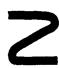
\includegraphics[keepaspectratio]{images/part002_5aba953c.jpg}}

In general, the dual of \(L^{\infty}\) is not isomorphic to \(L^{1}\) , consequently \(L^{1}\) and \(L^{\infty}\) are not reflexive (Exer. 10). We are going to characterize the continuous linear forms on \(L^{\infty}\) that arise, by passage to the quotient, from a linear form \(g \mapsto \int fg d\mu\) on \(L^{\infty}\) , where \(g \in L^{1}\) .

The ordered vector space \(\mathrm{L}^{\infty}(\mathrm{T},\mu)\) , which is a subspace of \(\mathrm{L}_{\mathrm{loc}}^{1}(\mathrm{T},\mu)\) , is fully lattice-ordered; for, if \((f_{\alpha})\) is a family of positive functions in \(L^{\infty}\) whose set of classes \((\dot{f}_{\alpha})\) is bounded above in \(L^{\infty}\) , there exists an \(a\geqslant0\) such that \(\mathrm{N}_{\infty}(f_{\alpha})\leqslant a\) for all \(\alpha\) . Since \(\mathrm{L}_{\mathrm{loc}}^{1}(\mathrm{T},\mu)\) is fully lattice-ordered, the family \((\dot{f}_{\alpha})\) admits a supremum \(\dot{h}\) in \(\mathrm{L}_{\mathrm{loc}}^{1}(\mathrm{T},\mu)\) ; but since \(\dot{a}\geqslant\dot{f}_{\alpha}\) for every \(\alpha\) , we have \(\dot{h}\leqslant\dot{a}\) , consequently \(\mathrm{N}_{\infty}(h)\leqslant a\) , whence our assertion.

PROPOSITION 14. --- In order that a positive linear form \(\theta\) on \(\mathcal{L}^{\infty}\) be of the type \(f \mapsto \int fg d\mu\) , where \(g \in \mathcal{L}^{1}\) , it is necessary and sufficient that, for every increasing directed family \((f_{\alpha})_{\alpha \in \mathrm{A}}\) of positive functions in \(\mathcal{L}^{\infty}\) whose set of classes \((\dot{f}_{\alpha})_{\alpha \in \mathrm{A}}\) is bounded above in \(\mathrm{L}^{\infty}\) and admits \(\dot{h}\) as its supremum in this space, one have

\[
\theta (h) = \sup _ {\alpha \in \mathrm{A}} \theta (f _ {\alpha}).
\]

Let us first show that the condition is necessary. The measure \(h \cdot \mu\) is the supremum in \(\mathcal{M}(\mathrm{T})\) of the set of measures \(f_{\alpha} \cdot \mu\) (No.~5, Scholium); therefore (Ch. II, §2, No.~2), for every function \(\varphi \geqslant 0\) in \(\mathcal{K}(\mathrm{T})\) , we have \(\int h\varphi d\mu = \sup_{\alpha \in \mathrm{A}} \int f_{\alpha}\varphi d\mu\) . If now \(a\) is a number \(\geqslant 0\) such that \(\mathrm{N}_{\infty}(f_{\alpha}) \leqslant a\) for all \(\alpha \in \mathrm{A}\) (which implies that \(\mathrm{N}_{\infty}(h) \leqslant a\) ), then for every \(\varepsilon > 0\) there exists a \(\varphi \in \mathcal{K}(\mathrm{T})\) such that \(\varphi \geqslant 0\) and \(\mathrm{N}_1(g - \varphi) \leqslant \varepsilon\) , from which we infer that \(\int f_{\alpha}|g - \varphi| d\mu \leqslant a\varepsilon\) for all \(\alpha \in \mathrm{A}\) , and \(\int h|g - \varphi| d\mu \leqslant a\varepsilon\) . Since \(\sup_{\alpha \in \mathrm{A}} \int f_{\alpha}g d\mu \leqslant \int hg d\mu\) , this proves that the two members of this inequality are equal.

To establish that the condition is sufficient, we shall make use of the following lemma:

Lemma 4. --- \(1^{\circ}\) Let \(f\) be a lower semi-continuous and bounded positive function on \(\mathbf{T}\) . Then its class \(\dot{f}\) in \(\mathbf{L}^{\infty}\) is the supremum of the set of classes \(\dot{\varphi}\) , where \(\varphi\) runs over the set of functions in \(\mathcal{K}(\mathbf{T})\) such that \(0 \leqslant \varphi \leqslant f\) .

\(2^{\circ}\) Let \(f\) be a measurable and bounded positive function on \(\mathbf{T}\) . Then its class \(\dot{f}\) in \(\mathrm{L}^{\infty}\) is the infimum of the set of classes \(\dot{\psi}\) , where \(\psi\) runs over the set of lower semi-continuous and bounded functions on \(\mathbf{T}\) that are \(\geqslant f\) .

\(1^{\circ}\) Let \(f'\) be a function in \(\mathcal{L}^{\infty}\) such that \(\dot{f}'\) is the supremum in \(\mathrm{L}^{\infty}\) of the set of classes \(\dot{\varphi}\) of the functions \(\varphi\) in \(\mathcal{K}(\mathrm{T})\) such that \(0 \leqslant \varphi \leqslant f\) ; obviously \(\dot{f}' \leqslant \dot{f}\) . Let U be a relatively compact open subset of T; for every function \(h\) in \(\mathcal{K}(\mathrm{T})\) such that \(0 \leqslant h \leqslant f\varphi_{\mathrm{U}}\) one has, by definition, \(h(t) \leqslant f'(t)\) locally almost everywhere, therefore \(h(t) \leqslant f'(t)\varphi_{\mathrm{U}}(t)\) almost everywhere; it follows that \(\int h d\mu \leqslant \int f'\varphi_{\mathrm{U}} d\mu\) . However, since \(f\varphi_{\mathrm{U}}\) is lower semi-continuous, \(\int f\varphi_{\mathrm{U}} d\mu = \sup \int h d\mu\) , where \(h\) runs over the set of functions in \(\mathcal{K}(\mathrm{T})\) such that \(0 \leqslant h \leqslant f\varphi_{\mathrm{U}}\) (Ch. IV, §1, No.~1, Def. 1); therefore

\[
\int f \varphi_ {\mathrm{U}} d \mu \leqslant \int f ^ {\prime} \varphi_ {\mathrm{U}} d \mu ,
\]

and since \(f' \varphi_{\mathrm{U}} \leqslant f \varphi_{\mathrm{U}}\) almost everywhere, necessarily \(f \varphi_{\mathrm{U}} = f' \varphi_{\mathrm{U}}\) almost everywhere, whence \(f = f'\) locally almost everywhere.

\(2^{\circ}\) Let \(f'\) be a function in \(\mathcal{L}^{\infty}\) such that \(\dot{f}'\) is the infimum in \(\mathrm{L}^{\infty}\) of the set of classes \(\dot{\psi}\) of the lower semi-continuous functions \(\psi\) that are bounded and \(\geqslant f\) ; then \(\dot{f}' \geqslant \dot{f}\) . Let K be a compact subset of T; for every lower semi-continuous function h that is bounded and \(\geqslant f\varphi_{K}\) , let \(\overline{h}\) be the function equal to h on K and to \(\|f\| + \|h\|\) on T - K. Then \(\overline{h}\) is lower semi-continuous and \(\geqslant f\) , therefore by definition \(\overline{h}(t) \geqslant f'(t)\) locally almost everywhere; it follows that \(h(t) \geqslant f'(t)\varphi_{\mathrm{K}}(t)\) almost everywhere, whence \(\int h d\mu \geqslant \int f'\varphi_{K} d\mu\) . But \(\int f\varphi_{K} d\mu = \inf \int h d\mu\) , where h runs over the set of lower semi-continuous functions that are bounded and \(\geqslant f\varphi_{K}\) (Ch. IV, §1, No.~3, Def. 3); therefore

\[
\int f \varphi_ {\mathrm{K}} d \mu \geqslant \int f ^ {\prime} \varphi_ {\mathrm{K}} d \mu ,
\]

and since \(f\varphi_{\mathrm{K}} \leqslant f'\varphi_{\mathrm{K}}\) almost everywhere, necessarily \(f\varphi_{\mathrm{K}} = f'\varphi_{\mathrm{K}}\) almost everywhere, whence \(f = f'\) locally almost everywhere.

The lemma having been proved, let \(\theta\) be a positive linear form on \(\mathcal{L}^{\infty}\) satisfying the condition in the statement of Prop. 14. The restriction of \(\theta\) to the space \(\mathcal{K}(\mathrm{T})\) is a positive measure \(\nu\) on \(\mathrm{T}\) . We are going to show that, for every positive function \(f\in \mathcal{L}^{\infty}(\mathrm{T},\mu)\) , one has \(\theta (f) = \nu^{*}(f)\) . Suppose first that \(f\) is lower semi-continuous (and bounded); by Lemma 4, \(\dot{f}\) is the supremum of the increasing directed set of classes \(\dot{\varphi}\) , where \(\varphi\) runs over the directed set \(\Phi\) of functions in \(\mathcal{K}(\mathrm{T})\) such that \(0\leqslant \varphi \leqslant f\) . Since by hypothesis \(\theta (f) = \sup_{\varphi \in \Phi}\theta (\varphi)\) , and \(\nu^{*}(f) = \sup_{\varphi \in \Phi}\nu (\varphi)\) by definition, our assertion is proved in this case. Secondly, suppose that \(f\) is \(\mu\) -measurable and bounded; then, by definition, \(\nu^{*}(f) = \inf_{\psi \in \Psi}\nu^{*}(\psi)\) , where \(\psi\) runs over the decreasing directed set \(\Psi\) of lower semi-continuous functions that are bounded and \(\geqslant f\) . If \(a\geqslant \| f\|\) then, applying the hypothesis of the statement to the increasing directed set of classes of the functions \(a - \psi\) , where \(\psi \in \Psi\) and \(\psi \leqslant a\) , one sees, by virtue of the lemma, that \(\theta (f) = \inf_{\psi \in \Psi}\theta (\psi)\) , therefore indeed \(\theta (f) = \nu^{*}(f)\) . In particular, for every \(\mu\) -negligible function \(f\geqslant 0\) , one has \(\theta (f) = 0\) , therefore \(\nu^{*}(f) = 0\) and consequently (No.~5, Th. 2) \(\nu\) is a measure with base \(\mu\) ; moreover, \(\nu^{*}(1) = \theta (1) < +\infty\) , consequently (Cor. of Th. 1) \(\nu = g\cdot \mu\) with \(g\in \mathcal{L}^1 (\mathrm{T},\mu)\) . Finally, since every \(\mu\) -measurable function is \(\nu\) -measurable, every positive function \(f\in \mathcal{L}^{\infty}(\mathrm{T},\mu)\) is \(\nu\) -integrable and \(\int fg d\mu = \nu^{*}(f) = \theta (f)\) , which completes the proof.

One concludes from Prop. 14 that the linear forms on \(\mathcal{L}^{\infty}\) of the type \(f\mapsto \int fg d\mu\) , where \(g\in \mathcal{L}^{1}\) , are the differences \(\theta_{1} - \theta_{2}\) , where \(\theta_{1}\) and \(\theta_{2}\) are positive linear forms satisfying the condition of Prop. 14.

